\section{Computation of FRFs}
\label{sec:computation_of_FRFs}

The computation of the FRFs is a crucial step in the analysis of the dynamic behavior of a structure.

The FRF is a complex-valued function that describes the steady-state response of a system to a sinusoidal excitation.
Even if the restriction over the shape of the excitation is quite severe, the FRF is a powerful tool to analyze the dynamic behavior of a system given that due to the linearity of the system, the response to a general excitation can be obtained by a linear combination of the responses to sinusoidal excitations (Fourier series).

By definition, the FRF is the ratio of the output to the input in the frequency domain.
For a linear time-invariant system, the FRF is a complex-valued function of the frequency, and it is defined as:

\begin{equation}
    H(\omega) = \frac{Y(\omega)}{X(\omega)}
\end{equation}

Where $H(\omega)$ is the FRF, $Y(\omega)$ is the Fourier transform of the output signal $y(t)$, and $X(\omega)$ is the Fourier transform of the input signal $x(t)$.

Moreover, to give a more practical definition, the FRF is the function that relates the output of a system considered at a specific coordinate to a sinusoidal input at a given coordinate.
If we then consider the system to be linear, time-invariant, and with a single input $@x_k$ and a single output $@x_j$, than the FRF can be defined as:

\begin{equation}
    H_{j,k}(\Omega) = \sum_{i=1}^{n} \frac{\Phi_i(x_j) \Phi_i(x_k) / m_i}{-\Omega^2 + 2\xi_i \omega_i \Omega i + \omega_i^2}
    \label{eq:FRF}
\end{equation}

Where, all the entities of Equation \ref{eq:FRF} are defined in Table \ref{tab:FRF_entities}.

\begin{table}[H]
    \centering
    \begin{tabular}{cl}
        \hline
        Parameter     & Description                                         \\
        \hline
        $\Phi_i(x^*)$ & Mode shape of the $i^{th}$ mode at coordinate $x^*$ \\
        $m_i$         & Equivalent mass of the $i^{th}$ mode                \\
        $\xi_i$       & Damping ratio of the $i^{th}$ mode                  \\
        $\omega_i$    & Natural frequency associated to the $i^{th}$ mode   \\
        $\Omega$      & Frequency of the sinusoidal excitation              \\
        \hline
    \end{tabular}
    \caption{Entities explanation for Equation \ref{eq:FRF}}
    \label{tab:FRF_entities}
\end{table}

As we can notice, among the entities of Equation \ref{eq:FRF}, at the moment we are only missing the equivalent mass $m_i$ and the damping ratio $\xi_i$.

The equivalent mass $m_i$ is a fictitious value that represents the amount of mass of the system that is effectively moving in the $i^{th}$ mode, weighted by the mode shape.
From this definition, we get:

\begin{equation}
    m_i = \int_{0}^{L} \rho A \Phi_i^2(x) dx
\end{equation}

For the damping ratio $\xi_i$, we can either use the Rayleigh damping model or the modal damping model.
However, since we are not dealing with a discretized system, but rather with a continuous one, for the sake of simplicity we will assume the damping ratio to be $\xi_i = \frac{c_i}{2 \sqrt{m_i k_i}} = 0.01$.

By doing so, we can compute the FRFs for the system at hand, and we can analyze the dynamic behavior of the structure.

\subsection{FRFs of the system due to a single point force}
\label{subsec:FRFs_of_the_system_due_to_a_single_point_force}

Once the FRFs function is defined, we can think of interrogate the structure to see how it reacts due to a single point force applied at a specific coordinate.

In particular, we can consider a sinusoidal force applied at coordinate $x_k = 0.9m$ and see how the structure reacts at a set of coordinates $x_j = [0.2 \quad 0.4 \quad 0.6 \quad 0.8 \quad 1.0 \quad 1.2]m$.
A graphical representation of the considered situation can be seen in Figure \ref{fig:beam_single_point_force}.

\begin{figure}[H]
    \centering
    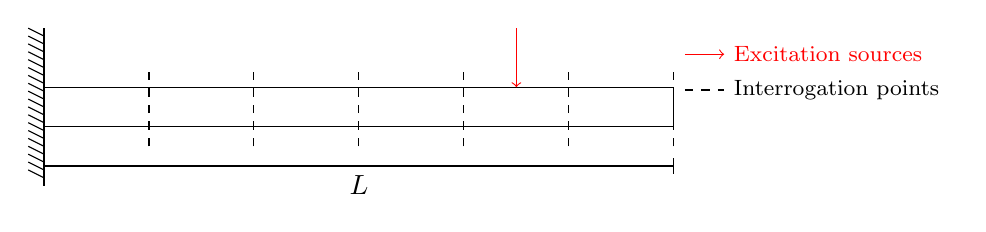
\begin{tikzpicture}[xscale=1, yscale=0.5]

        \draw (0,-0.5) rectangle (8, 0.5);
        \draw[|-|] (0, -1.5) -- (8, -1.5) node[midway, below]{$L$};

        \draw (0, -2) -- (0,  2);

        \foreach \y in {-1.8, -1.6, ..., 1.8}
        \draw (0, \y) -- ++(-0.2, +0.2);

        \foreach \x in {0.2, 0.4, ..., 1.2}
        \draw[dashed] (\x * 8/1.2, -1.0) -- ++(0.0, +2.0);

        \draw[<-, red] (0.9 * 8/1.2, 0.5) -- ++(0.0, +1.5);

        % Add legend
        \node [matrix, font = \footnotesize, below right, row sep = 0cm] at (current bounding box.north east)
        {
            \draw[->, red] (0, 0) -- ++(0.5, 0) node[right, red] {Excitation sources}; \\
            \draw[dashed, black] (0, 0) -- ++(0.5, 0) node[right, black] {Interrogation points}; \\
        };

    \end{tikzpicture}
    \caption{Analyzed situation: single input, multiple outputs}
    \label{fig:beam_single_point_force}
\end{figure}

Since we are now considering $6$ different coordinates, we will have $6$ different FRFs, each one describing the response of the structure at a specific coordinate due to the excitation $f(t) = F_0 \sin(\Omega t) = 1 \sin(\Omega t)$.

By doing so, we obtain the module and phase plots reported in Figure \ref{fig:FRFs_single_point_force}.

\begin{figure}[H]
    \centering
    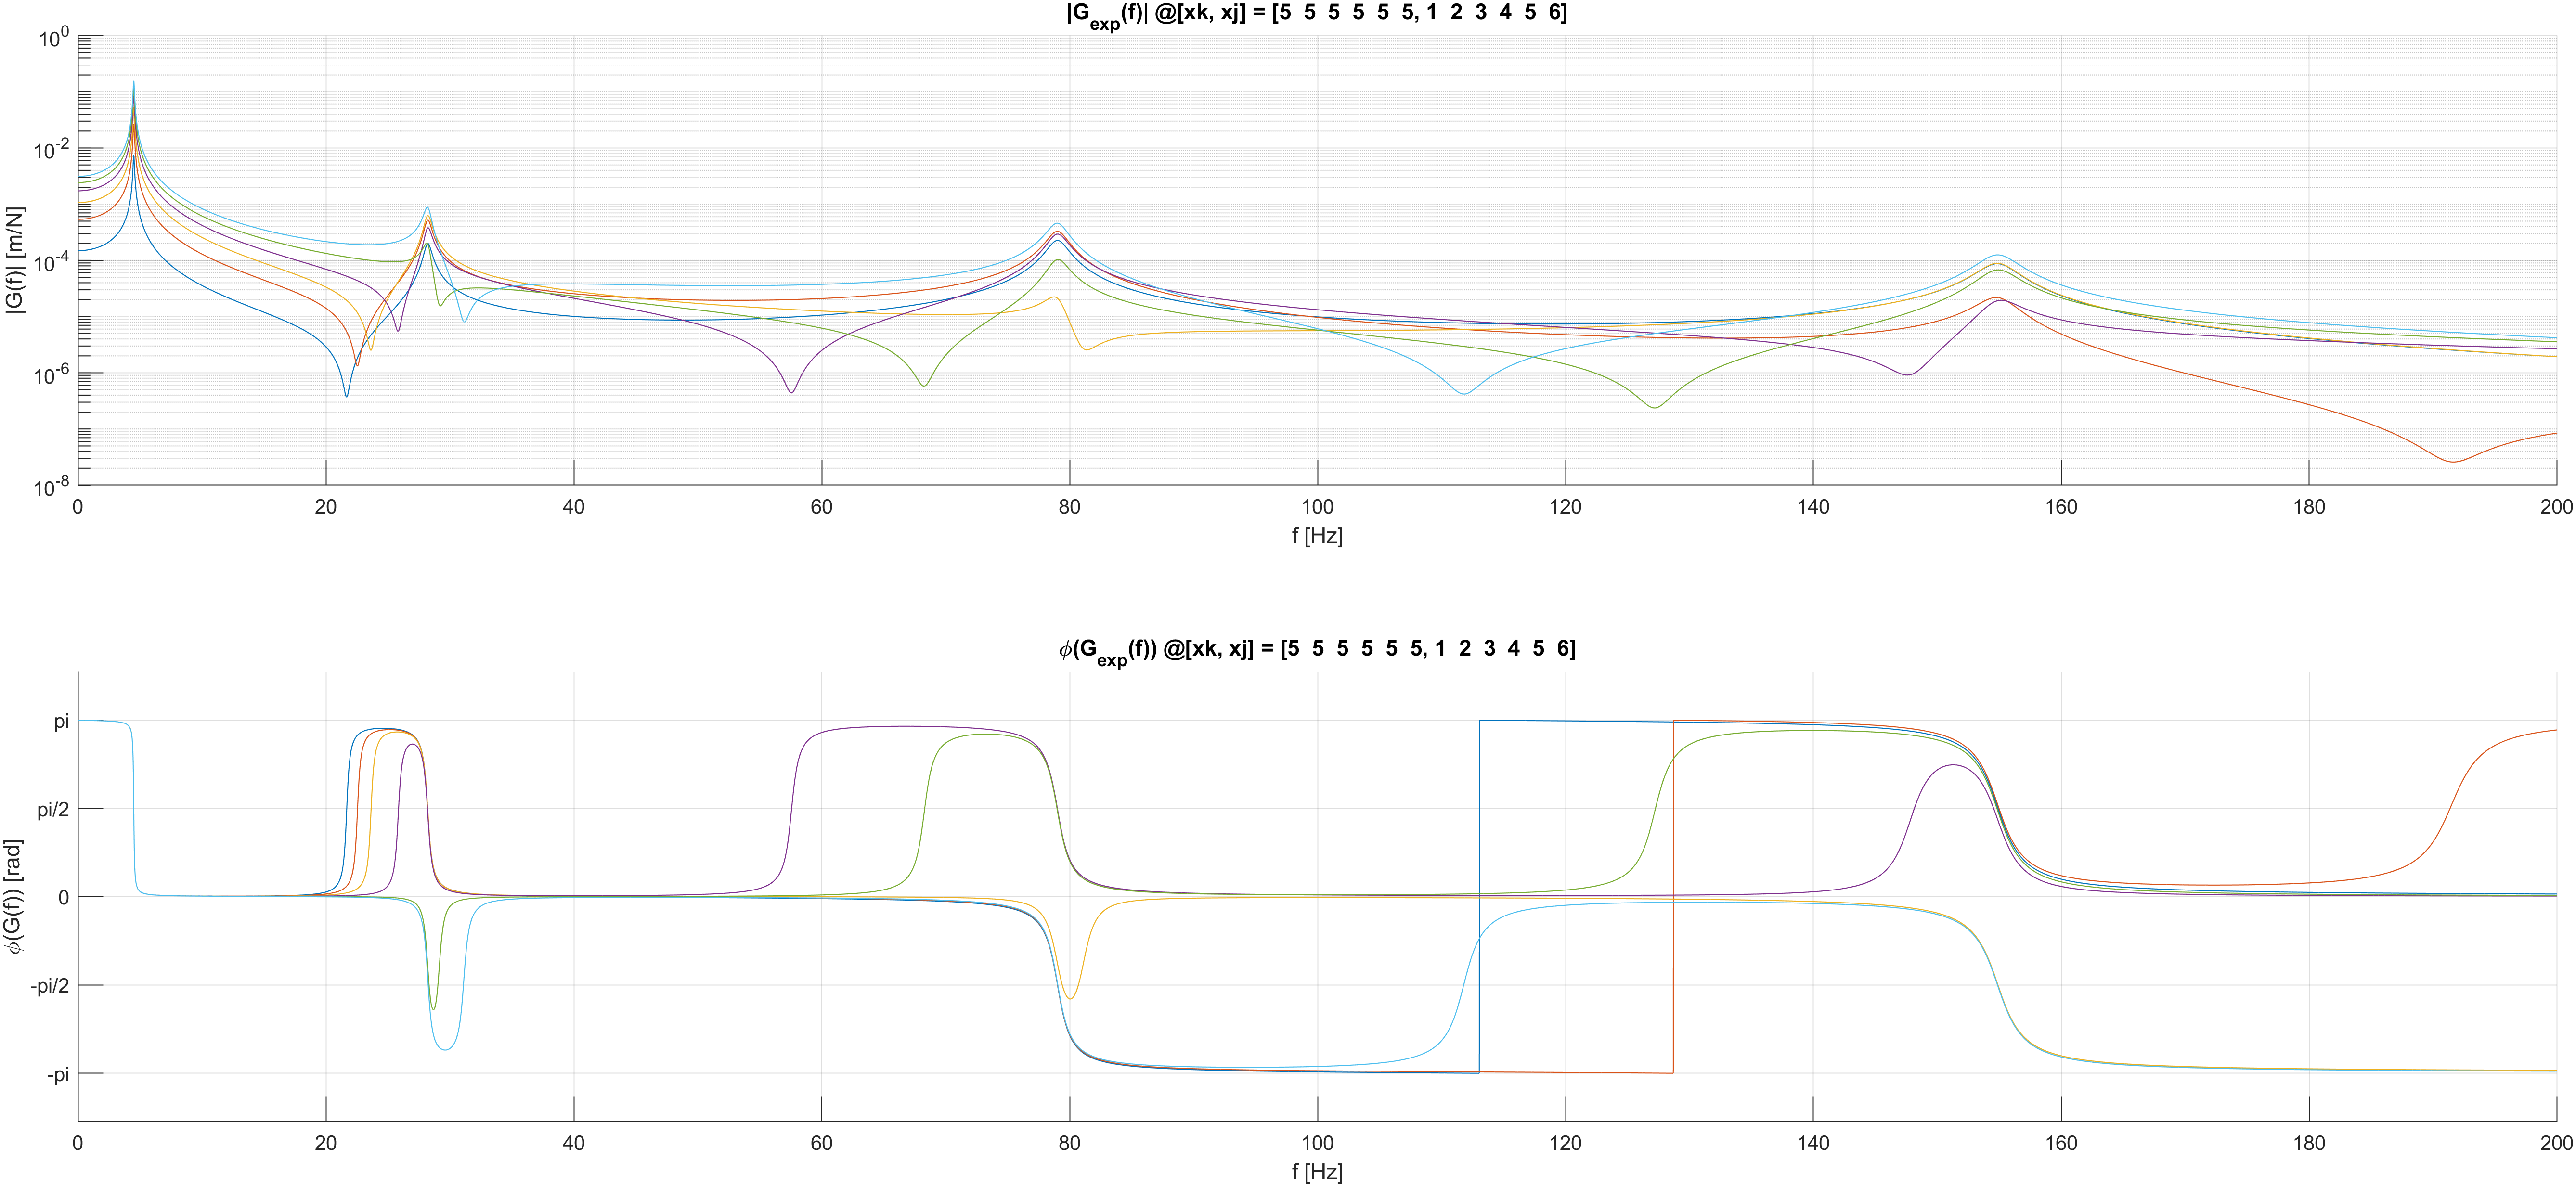
\includegraphics[width=\textwidth]{img/MATLAB/Part_A/Experimental_FRF_SIMO.png}
    \caption{FRFs of the system due to a single point force. Each color in the plot represents the FRF of the structure at a specific output coordinate.}
    \label{fig:FRFs_single_point_force}
\end{figure}

\subsection{FRFs of the system due to a multiple point force}
\label{subsec:FRFs_of_the_system_due_to_multiple_point_force}

The next step is to observe the behavior of the structure when multiple forces are applied to it.

As we have said in the previous section, even if the FRF given information about a single input and a single output, we can still use it to understand how the structure behaves when multiple forces are applied to it and study the structural response at different coordinates.

For the sake of simplicity, we will consider a structure with $2$ excitation points at $x_k = [0.3 0.9]m$ and $3$ output points at $x_j = [0.2 0.8 1.2]m$.

A graphical representation of the considered situation can be seen in Figure \ref{fig:beam_multi_point_force}.

\begin{figure}[H]
    \centering
    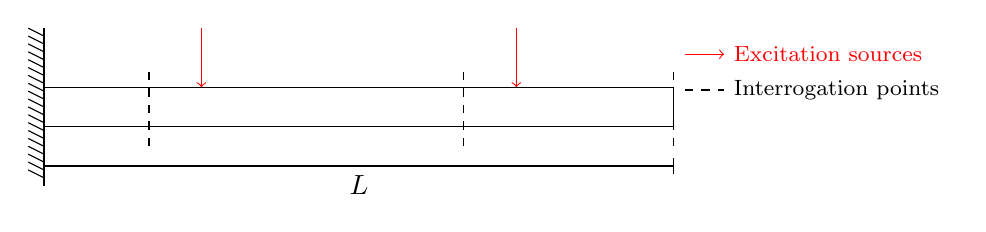
\begin{tikzpicture}[xscale=1, yscale=0.5]

        \draw (0,-0.5) rectangle (8, 0.5);
        \draw[|-|] (0, -1.5) -- (8, -1.5) node[midway, below]{$L$};

        \draw (0, -2) -- (0,  2);

        \foreach \y in {-1.8, -1.6, ..., 1.8}
        \draw (0, \y) -- ++(-0.2, +0.2);

        \foreach \x in {0.2, 0.8, 1.2}
        \draw[dashed] (\x * 8/1.2, -1.0) -- ++(0.0, +2.0);

        \foreach \x in {0.3, 0.9}
        \draw[<-, red] (\x * 8/1.2, 0.5) -- ++(0.0, +1.5);

        % Add legend
        \node [matrix, font = \footnotesize, below right, row sep = 0cm] at (current bounding box.north east)
        {
            \draw[->, red] (0, 0) -- ++(0.5, 0) node[right, red] {Excitation sources}; \\
            \draw[dashed, black] (0, 0) -- ++(0.5, 0) node[right, black] {Interrogation points}; \\
        };

    \end{tikzpicture}
    \caption{Analyzed situation: multiple inputs, multiple outputs}
    \label{fig:beam_multi_point_force}
\end{figure}

Similar reasoning as before can be done about the expected result of this type of analysis in terms of number of FRFs to be computed and the information that can be extracted from them.

Moreover, given that we are now dealing with a multi-input system, the actual displacement of the structure at a specific coordinate will be the result of the superposition of the displacements due to each excitation force.

Before proceeding with the visualization of the actual FRFs, it's important to stress that what we are actually "superposing" are the complex FRFs, not only their modules.
This means that the phase information is also taken into account when computing the total response of the structure.
But also remember that the phase information is also dependent on the phase of the input force, so it's important to keep track of it when analyzing the results.

To better understand this aspect, we can move on a complex plane and consider the output of a generic system due to two different input forces $F_1 = F_{1,0} \sin(\omega_1 t + \phi_1)$ and $F_2 = F_{2,0} \sin(\omega_2 t + \phi_2)$.

\begin{figure}[H]
    \centering
    \begin{tikzpicture}[scale=0.8]

        \coordinate (O) at (0, 0);
        \coordinate (A) at (2, 1);
        \coordinate (B) at (-3, 1);
        \coordinate (C) at (3, -2);
        \coordinate (D) at (-2, 4);

        \draw[->] (-4,0) -- (4,0) node[right] {Re};
        \draw[->] (0,-4) -- (0,4) node[above] {Im};

        \draw[->, thick, red] (O) -- (A) node[midway, above, sloped] {$F_1$};
        \draw[->, thick, red] (O) -- (B) node[midway, above, sloped] {$F_2$};
        \draw[->, thick] (O) -- (C) node[midway, above, sloped] {$FRF_1$};
        \draw[->, thick] (O) -- (D) node[midway, above, sloped] {$FRF_2$};

        \pic [draw, <-, "$\phi_{FRF1}$", angle radius = 2cm] {angle = C--O--A};
        \pic [draw, <-, "$\phi_{FRF2}$", angle radius = 1cm] {angle = D--O--B};

    \end{tikzpicture}
    \hfill
    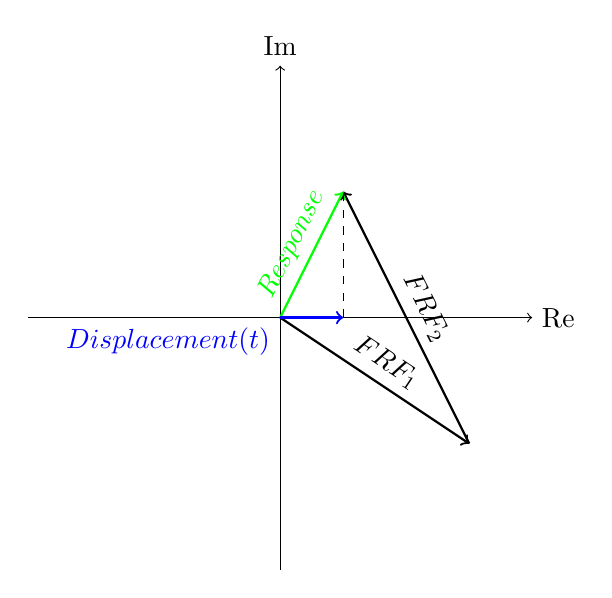
\begin{tikzpicture}[scale=0.8]

        \coordinate (O) at (0, 0);
        \coordinate (A) at (2, 1);
        \coordinate (B) at (-3, 1);
        \coordinate (C) at (3, -2);
        \coordinate (D) at (-2, 4);

        \draw[->] (-4,0) -- (4,0) node[right] {Re};
        \draw[->] (0,-4) -- (0,4) node[above] {Im};

        \draw[->, thick] (O) -- (C) node[midway, above, sloped] {$FRF_1$};
        \draw[->, thick] (C) -- ++(D) node[midway, above, sloped] {$FRF_2$};

        \draw[->, thick, green] (O) -- (1, 2) node[midway, above, sloped] {$Response$};
        \draw[dashed] (1, 0) -- (1, 2);
        \draw[->, thick, blue] (O) -- (1, 0) node[below left] at (O) {$\text{Displacement}(t)$};



    \end{tikzpicture}
    \caption{Complex plane representation of the FRFs of the system due to multiple input forces and the actual displacement of the output/interrogation point.}
    \label{fig:complex_plane_representation}
\end{figure}

As is clearly see in Figure \ref{fig:complex_plane_representation}, the actual displacement of the output point can in some cases (or better for some period of time) be definitely lower than the sum of just the absolute modules of the FRFs.

If we came back and considering again the situation represented in Figure \ref{fig:beam_multi_point_force}, we obtain the module and phase plots reported in Figure \ref{fig:FRFs_multi_point_force}.

\begin{figure}[H]
    \centering
    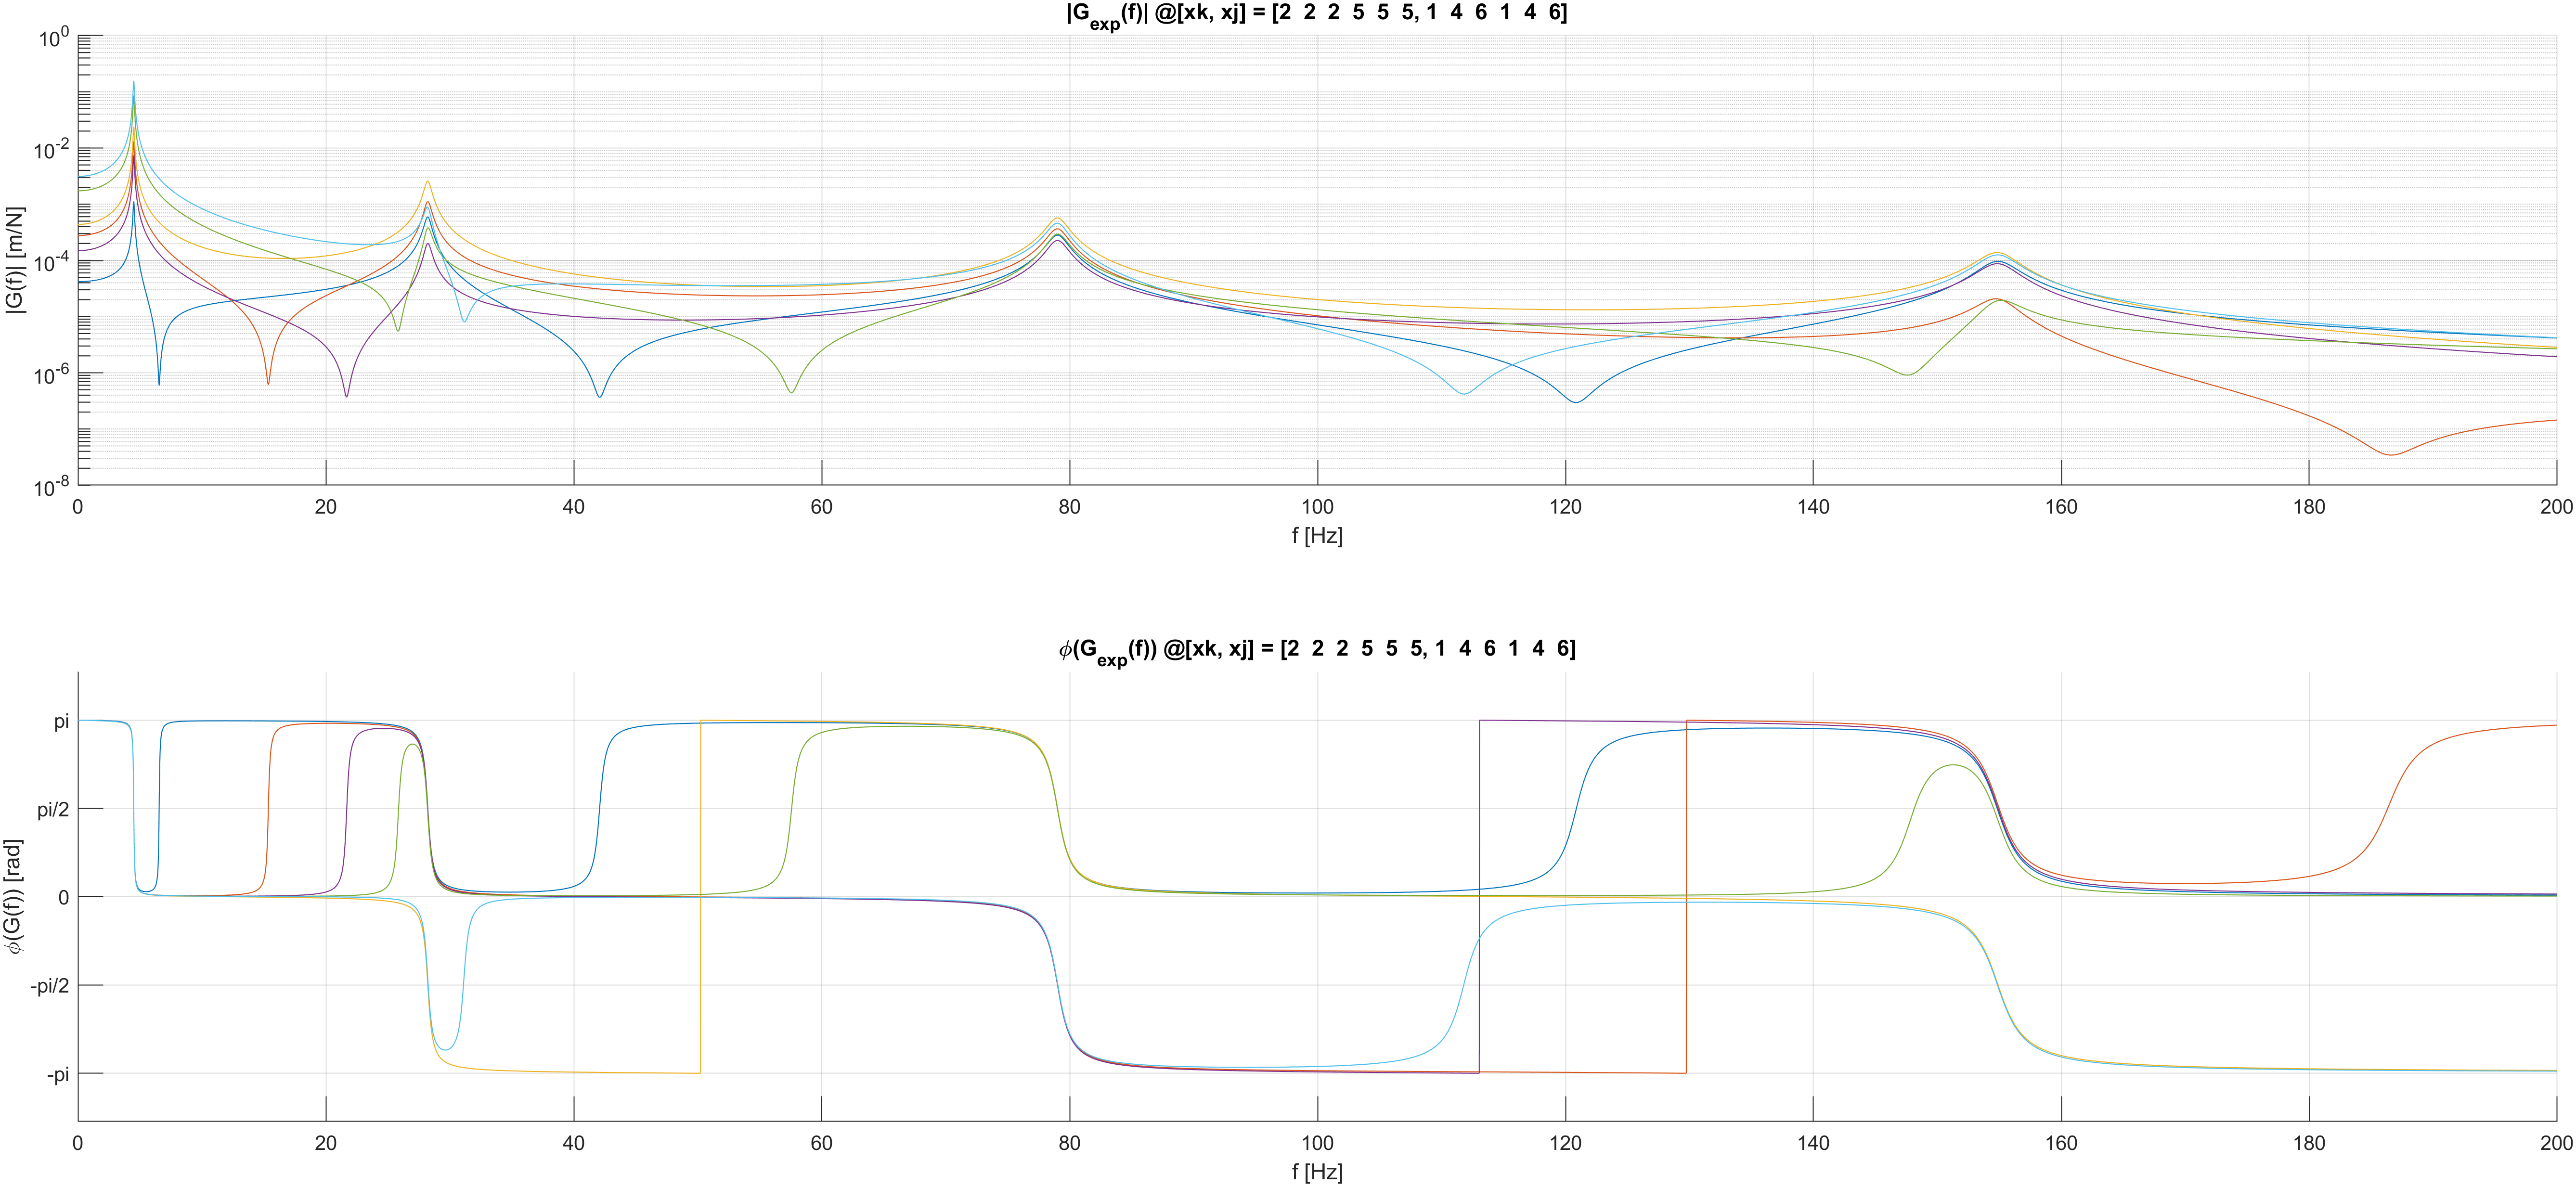
\includegraphics[width=\textwidth]{img/MATLAB/Part_A/Experimental_FRF_MIMO.png}
    \caption{FRFs of the system due to a couple of point force. Each color in the plot represents the FRF of the structure at a specific output coordinate.}
    \label{fig:FRFs_multi_point_force}
\end{figure}
